\section{Requirements}
\label{sec:Requirements}
Initially, this project was conceived by Dr. Kenny Hunt, who is served as the advisor, and almost all of the requirements were given by him, in an introductory meeting. Both the advisor, who is also the project sponsor, and the developer, who is also the author, are the stakeholders of the project.

After that, the advisor met with the developer almost every workday to gather informal functional requirements of this project, he would also refine any previous requirements that were given. These requirements played a crucial role in the development of the map generator. On the one hand, the scope of development was clarified, and on the other hand, the necessary algorithms were compiled to maintain the continuation of development.

\subsection{Functional Requirements}
The functional requirements focus on developing a web application. There are two roles for this system: ``admins'' and ``users''. As a result, the following functional requirements were established for the project:
\begin{enumerate}
  \item As an admin or a user, I need to be able to:
  \begin{enumerate}
    \item Log In: with unique email and password
    \item Log Out: end the session
    \item Edit Personal Profile: change email, first name, last name, and password
  \end{enumerate}
  \item As an admin, I want to be able to:
  \begin{enumerate}
    \item View All Users: on the ``dashboard'' page
    \item Enable or Disable Users: allow the user to log in or not
    \item Search for Users: use any combination of email, first name, and last name; on the ``dashboard'' page
  \end{enumerate}
  \item As a user, I want to be able to:
  \begin{enumerate}
    \item Sign Up: with unique email, first name, last name, long password, and confirmed password
    \item View All Own Maps: on the ``dashboard'' page
    \item View All Visible Maps: on the ``community'' page
    \item Search for Maps: use any combination of the map name, created date, edited date, the owner's email, the owner's first name, and the owner's last name; on the ``community'' page
    \item Download Maps: of either your own or other visible maps; in ``png'' or ``svg'' format
    \item Make Maps Public or Private: allow the map displaying on the ``community'' page or not
    \item Create Maps: with a name; on the ``dashboard'' page
    \item Delete Maps: on the ``dashboard'' page
    \item Edit Maps:
    \begin{enumerate}
      \item When the user opens the map editor page, it shows an empty map with random map seeds by default, and then the user can make maps by accessing the menu on the right
    	\item In the menu, the user can input the number of map seeds to create a new empty map
    	\item The user can select different types of layers for the map: elevation, affluence, desirability, district, and building, which can superimpose on each other
      \item The user can choose to display street names or not
      \item The user can manipulate the ``increase/decrease toggle,'' ``increment sliding,'' and ``waterline sliding'' to edit the map: increasing or decreasing the value of elevation and affluence; building or removing the wall; making map cell as water or city
      \item If the waterline is changed, the continent will be changed accordingly
      \item The user can choose to display contour lines or not
      \item After selecting one or more than one layers under ``edit'' mode, the user can change the size of the "soft brush" by using the mouse wheel, which determines the area where the map will be edited
      \item The user edits the map by clicking and dragging the ``soft brush.''
      \item The districts and buildings are procedurally generated
      \item The user is allowed to change the type of the current district by right-clicking and selecting a new type from the context menu
      \item The map provides 13 different types of districts: rich, medium, poor, empty, plaza, park, farm, water, harbor, university, religious, castle, and military
      \item The user can zoom in and zoom out the map by pressing on the alt key and using the mouse wheel
      \item The user can use a specialized button to resize the map on the right top
      \item The user can save the map or download it by clicking the button on the right bottom
    \end{enumerate}
  \end{enumerate}
\end{enumerate}

Figure \ref{Use Case Diagram} is the use case diagram that describes the functionalities to be implemented by this web application.

\begin{figure}[htbp]
\centering
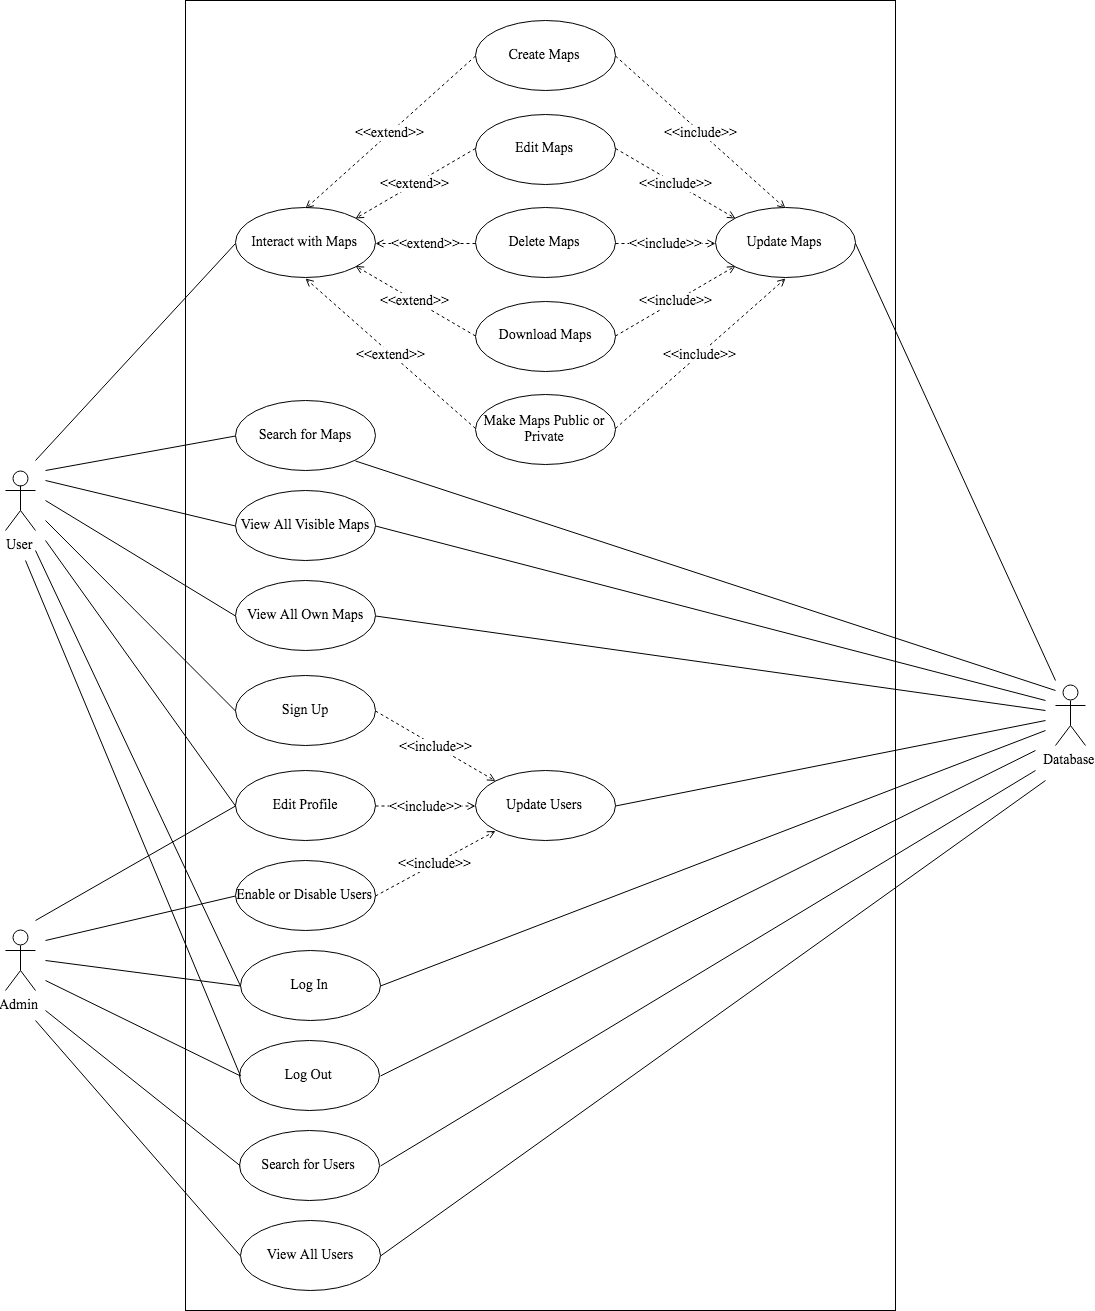
\includegraphics[width=\textwidth]{section02/assets/use_case.png}
\caption[Use Case Diagram]{\label{Use Case Diagram}Use Case Diagram}
\end{figure}

\subsection{Non-Functional Requirements}
There are numerous non-functional requirements of a system: response time, availability, usability, security (authentication, authorization, integrity, privacy, etc.), and so on. For this application, we decided to focus on the following requirements:
\begin{enumerate}
  \item Security:
  \begin{enumerate}
    \item Input Validation:
    \begin{enumerate}
      \item Add validations at both client and server sides
      \item All methods should always validate all parameters in the server-side
    \end{enumerate}
    \item Password Encryption:
    \begin{enumerate}
      \item Shall always be encrypted
      \item Not even the system administrators shall see clear text passwords
      \item Applying a hashing algorithm to passwords
    \end{enumerate}
    \item Prohibiting Cross Site Scripting (XSS):
    \begin{enumerate}
      \item Never insert data anywhere in a ``script'' element
      \item Never insert data in an HTML comment
      \item Never insert data anywhere in CSS
      \item Never insert data in an attribute name
      \item Never insert data in an attribute value
      \item Never insert data in a tag name
    \end{enumerate}
    \item Secure Session Cookie:
    \begin{enumerate}
      \item Set the ``Secure'' cookie attribute and instruct web browsers to send the cookie only over encrypted, e.g., HTTPS, links.
      \item Set the ``HttpOnly'' attribute true and prohibiting the JavaScript code from reading the cookie via the DOM ``document.cookie'' JavaScript object.
      \item Always change the session id after login
    \end{enumerate}
  \end{enumerate}
  \item Performance:
  \begin{enumerate}
    \item High performance of rendering map:
    \begin{enumerate}
      \item Compare and select the most appropriate and the fastest way to render maps, e.g., canvas, SVG
    \end{enumerate}
  \end{enumerate}
\end{enumerate}

\subsection{Selection of Software Development Life Cycle Model}
We analyzed and summarized the following possible risks:
\begin{enumerate}
  \item Lack of experience developing in a map generation
  \item The certainty whether a third-party library was available as the map rendering engine
  \item The potential misunderstanding between the advisor and the developer with respect to the requirements
\end{enumerate}

To reduce or avoid these risks, two life cycle models were considered in the beginning: waterfall and agile. Because of the daily meeting between the advisor and the author, and there will be new requirements almost every time. The waterfall model is beyond our consideration. Unlike the waterfall model, we only need initial planning to start this project, and every time the new requirements are almost based on the previous one. Finally, the agile model was chosen, which is shown in Figure \ref{Agile Model}.

\begin{figure}[htb]
\centering
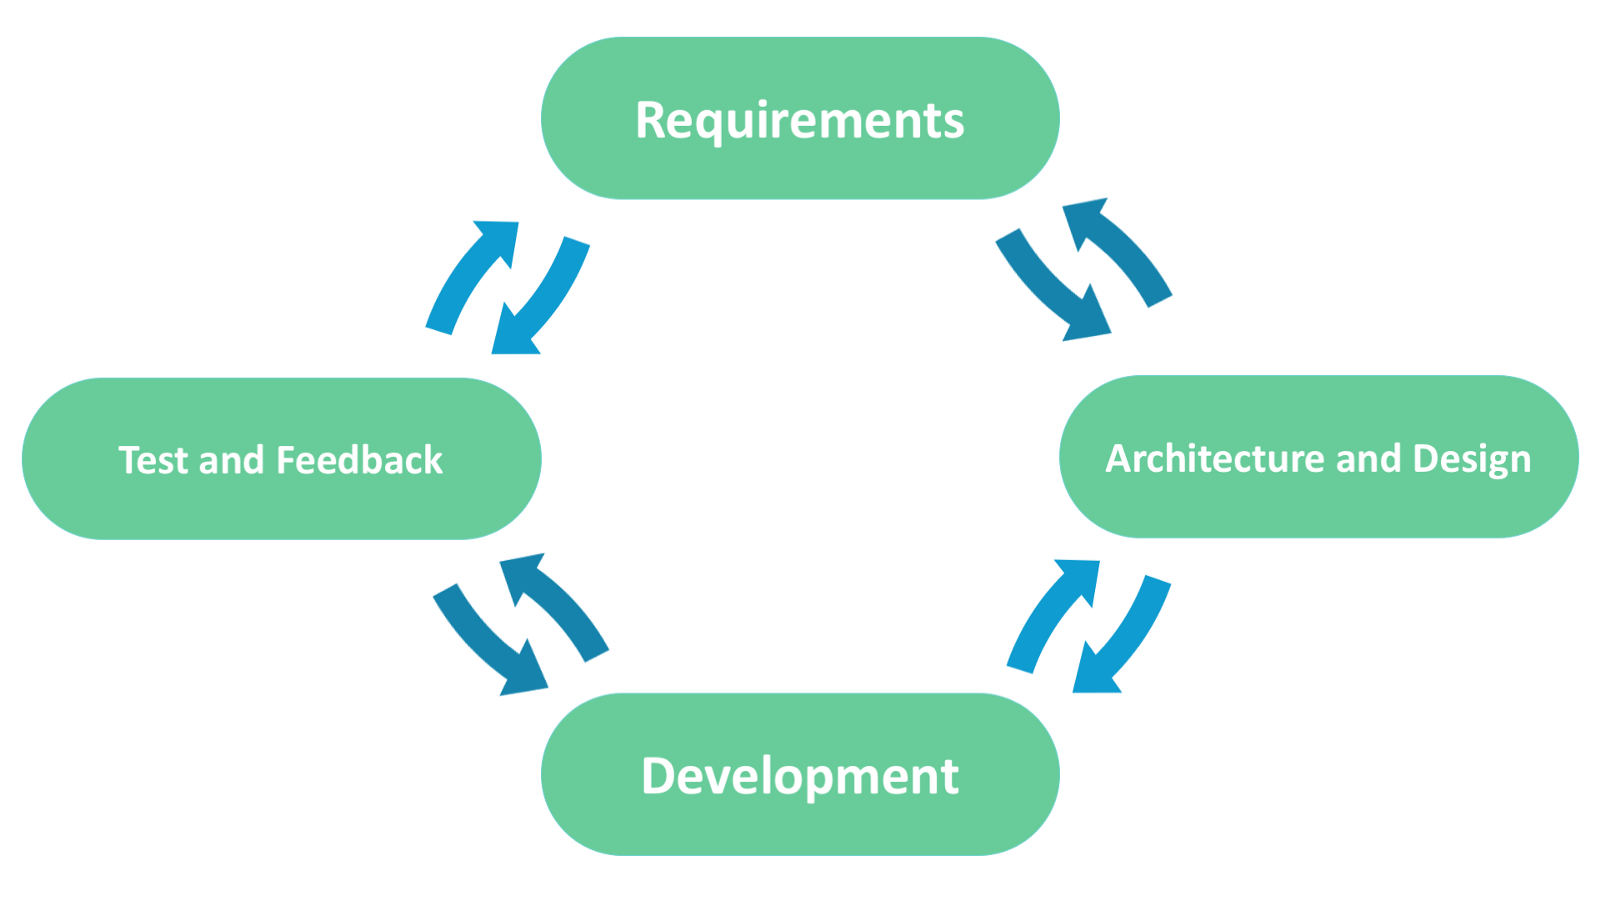
\includegraphics[width=\textwidth]{section02/assets/agile.png}
\caption[Agile Development Life Cycle Model]{\label{Agile Model}Agile Development Life Cycle Model}
\end{figure}

Agile methodology is a practice that helps continuous iterations of development and testing in the software development process. In this model, development and testing activities are concurrent. Unlike the waterfall model, this process allows more communications between the advisor and the developer. Furthermore, the agile model is a combination of iterative and incremental process models. Agile methods break the product into small incremental builds. These builds are provided in iterations. Each iteration typically lasts from about one to three weeks. The iterations that have occurred in
this project are listed below:
\begin{enumerate}
  \item Iteration 1: Change third-party libraries to generate maps
  \item Iteration 2: Change entirely and procedurally generated maps to partially and manually generated
  \item Iteration 3: Migrate codes from demo to the main project
  \item Iteration 4: Improve the performance of rendering maps
\end{enumerate}
At the end of the iteration, a working product demo is displayed to stakeholders. There are several known advantages and disadvantages of using the agile model in this project:
\begin{enumerate}

  \item Advantages:
  \begin{enumerate}
    \item Easy to manage
    \item Little or no planning required
    \item Gives flexibility to developers
    \item Resource requirements are minimum
    \item Suitable for fixed or changing requirements
  \end{enumerate}

  \item Disadvantages:
  \begin{enumerate}
    \item More risks of sustainability, maintainability, and extensibility
    \item An overall plan, an agile leader (the advisor) is a must without which it will not work
    \item There is a very high individual dependency since there is minimum documentation generated
  \end{enumerate}

\end{enumerate}
